\chapter{Technical details of uDrone System} \label{system}
This section will list the requirements for the uDrone system along with the chosen hardware components and software tools used to meet them.
\section{System Requirements}
Based on the science needs and goals of building a testbed, several design requirements emerged.
\subsection{Science Requirements}
\begin{itemize}
    \item Maintain a constant speed of 1 m/s.
    \item Maintain a constant distance from the reef, ideally between 30 and 100 cm.
    \item Know the exact distance to the reef to calibrate spectrography readings.
    \item Operate for at least 4 hours.
    \item Be able to carry the necessary spectrography equipment and light source.
    % \item “Field spectra were measured using an ASD HandHeldPro-2 spectrometer with an underwater housing and tungsten halogen light source at a distance of 10 cm from the benthic targets (live coral, bleached coral, etc.) (Appendix A, Figure A2). (cite: Li sensitivity…)
    \item Travel fully autonomously, with no tether or human control.
    \item Maintain a straight line path underwater.
    \item GPS tag the start and end locations in order to estimate the exact locations of all measurements in-situ.
    \item Be deployed and retrieved by one or two people from the shore or a small boat. 
\end{itemize}

\subsection{Testbed Requirements}
\begin{itemize}
    \item Use ROS and PX4 as open source frameworks.
    \item GPU to allow for on board machine learning and neural networks.
    \item Sensors to generate local awareness for navigation.
    \item Cost less than \$10,000.
    \item Easy access to internal components.
    \item Each component replaceable or upgradable.
    \item Code can be tested in a robust simulation environment.
\end{itemize}

\begin{figure}[h]
\centering
\subfigure{\includegraphics[width=0.35\linewidth]{img/side.png}}
\subfigure{\includegraphics[width=0.28\linewidth]{img/front.png}}
\subfigure{\includegraphics[width=0.34\linewidth]{img/ortho.png}}
\caption[Side, front, and orthogonal view of the uDrone]{Side (left), front (center), and orthogonal (right) view of the uDrone}
\label{3ways}
\end{figure}

\section{Hardware Components}
The hardware components were chosen to be easy to obtain and mimic the construction of autonomous aerial vehicles as much as possible. The  physical and logical connections of the uDrone system is diagramed in Figure \ref{system_diagram}. In this diagram the blue boxes represent physical components, the red boxes represent software frameworks, the solid lines represent physical connections, and the dashed lines represent logical connections. The specific components listed here are discussed in the remainder of this chapter. 

\begin{figure}[h]
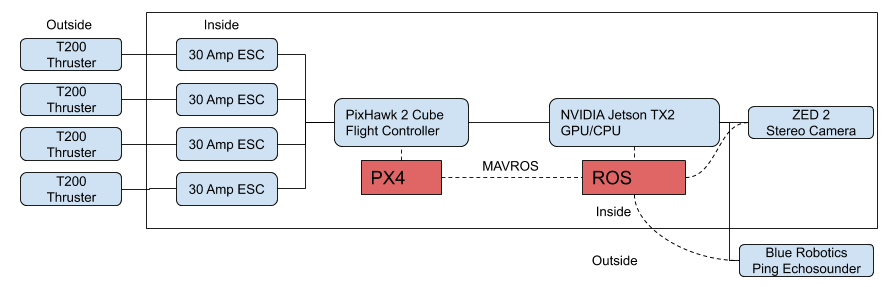
\includegraphics[width=\maxwidth{\textwidth}]{img/uDrone System Diagram.png}
\caption{uDrone System Diagram}
\label{system_diagram}
% \legend{\emph{Source}: \iftoggle{usebiblatex}{\textcite{krishnappa_adult_2012}}{\citet{krishnappa_adult_2012}}}% See: https://upload.wikimedia.org/wikipedia/commons/8/89/Antidorcas_marsupialis%2C_male_%28Etosha%2C_2012%29.jpg
% \legend{\emph{Note}: Here is a note that is especially long to show what happens when it extends to more than one line.}
\end{figure}



\subsection{Blue Robotics T200 Thrusters}
% https://bluerobotics.com/store/thrusters/t100-t200-thrusters/t200-thruster/
% https://discuss.bluerobotics.com/t/t200-high-voltage-behavior/94/4 (lifespan)

Blue Robotics is a leading source for marine robotics components. Arising from a kickstarter in 2014, they are DREAMS Lab’s preferred vendor for many components. Their thrusters fit the uDrone’s needs quite well, including their size, power usage, thrust capabilities, depth limits, and price. Additionally, as these are sold commercially it is very easy to have spares and order more on short notice. Given how perfectly these thrusters fit the requirements, no other thruster was seriously considered. One potential drawback to these thrusters is the expected lifetime of 600-1000 hours \parencite{t200}. While for some long range missions this would be a problem, with a mission time of only a few hours this poses no risks to the uDrone. 

The thrusters are controlled via a 30 amp electronic speed controller (ESC). This device modulates the power to the device based on pulse width modulation (PWM) signals it receives from the flight controller. 

\subsection{PixHawk 2 Cube Black}

% https://docs.px4.io/v1.9.0/en/flight\_controller/pixhawk-2.html
% http://www.proficnc.com/all-products/31-pixhawk2-suite.html

The DREAMS Lab uses PixHawk flight controllers for most aerial and aquatic robotics applications. Due to the experience and expertise with this piece of equipment, the same type of flight controller is used for the uDrone. The cube was chosen over newer PixHawks, like the PixHawk 4 mini, because it is more widely used in the PX4 community and the smaller size was not needed for the uDrone implementation.

The PixHawk 2 Cube runs PX4 on the NuttX operating system. It has multiple built-in three-axis gyroscopes, accelerometers, and magnetometers along with barometers, forming redundant internal measurement units (IMUs). It communicates with the on-board computer via MAVLINK messages over a serial connection. These messages are generated on the on-board computer from the MAVROS package. The PixHawk is able to control the motors via PWM outputs. 

These PixHawk devices typically run either PX4 or ArduPilot. Due to DREAMS Lab’s expertise, along with the related work being done, PX4 is used for the uDrone. The PX4 software has several different flight modes, including position, altitude, acrobatic, and manual control. The uDrone uses the acrobatic mode controlled via the on-board computer. In this mode the controller receives the desired orientation or angular rate along with a thrust value. Utilizing the internal IMUs, a built in PID controller takes these inputs and sends the desired PWM command to each motor \parencite{px4_pixhawk}. 

% \begin{itemize}
%     \item An STM32F427 Rev 3 Flight management unit
%     \item An STM32F100 I/O processor with pass through capabilities for failsafe
%     \item 3 IMU's
%     \item 1 Fixed 10 Axis IMU on the main Main board
%     \item 2 Vibration Isolated and heat controlled 9DOF IMU's and an isolated Barometer
% \end{itemize}

\subsection{Jetson TX2 with Connecttech Orbit Carrier}
% https://developer.nvidia.com/embedded/jetson-tx2
% https://connecttech.com/product/orbitty-carrier-for-nvidia-jetson-tx2-tx1/
% https://developer.nvidia.com/embedded/jetpack
The on board computer is an NVIDIA Jetson TX2. This device has a 256-core NVIDIA Pascal™ GPU along with a Quad-Core ARM® Cortex®-A57 MPCore \parencite{tx2}. The ARM processor is used to run ROS while the GPU is used to run neural-networks and process imagery on board. This device is specifically made for embedded systems and robotic applications. The TX2 runs on a Linux kernel with NVIDIA’s JetPack SDK \parencite{jetpack}.

To make interfacing with the TX2 easier, it is purchased with a Connect Tech Orbitty Carrier. The board connects to the TX2 module and provides computer style connectors, such as HDMI and Ethernet \parencite{orbitty}. This allows for easy interfacing with the TX2 for development and testing purposes. 

The NVIDIA Jetson TX2 is specifically built to be used with embedded robotic systems. The product’s tagline is “The AI Platform for Autonomous Machines.” This device has already been used for on board applications in autonomous underwater vehicles \parencite{MandersonGPU}.  Given its form factor, capabilities, and previous uses in related fields, this was chosen over other on board AI products for use in the uDrone. 

\subsection{ZED 2}
% https://www.stereolabs.com/ZED-2/

The StereoLabs ZED 2 was chosen as a stereo depth camera, and can be clearly seen in the center view of figure \ref{3ways}. StereoLabs specializes in AI-enabled stereo cameras. The ZED 2, their newest offering, has an internal IMU, barometer, and magnetometer to increase its visual servoing and depth-sensing abilities. The ZED 2 can also run neural networks on board to accomplish things like person tracking \parencite{zed}. While this feature is not used at the moment on the uDrone, it could be used with the implementation of other neural networks, such as fish identification and tracking. ZED cameras also integrate directly into ROS, making incorporating them into the system easier. An example of the output from the ZED 2 stereo camera while the uDrone is undergoing a pool test can be seen in figure \ref{stereo}.

\begin{figure}[ht]
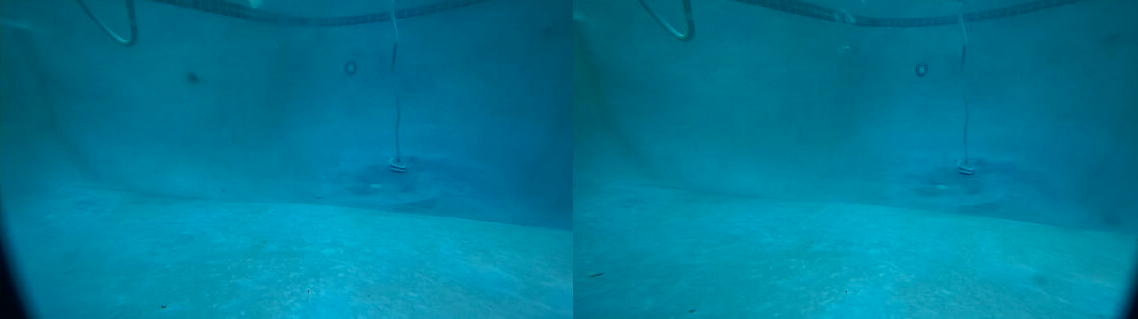
\includegraphics[width=\maxwidth{\textwidth}]{img/zed_pool.png}
\caption{Stereo Camera Output from ZED 2 in uDrone Pool Test}
\legend{\emph{Source}: Photo courtesy of Jnaneshwar Das, used with permission.}
\label{stereo}
\end{figure}

% ***Write the next part after results from JD
% Because light moves differently underwater (expand) the ZED 2 needed to be recalibrated to work underwater. ***DO more here in the future***
% Orientation?
% First go is front facing
% Do we need to do some tests with downward-facing?

\subsection{Blue Robotics Ping Echosounder}
% https://bluerobotics.com/store/sensors-sonars-cameras/sonar/ping-sonar-r2-rp/

The Blue Robotics Ping is a single beam echosounder for measuring distance underwater on the uDrone. It is attached in a downward facing orientation, allowing it to tell the distance of the uDrone to the reef. By aligning it in the same direction as the hyper-spectral sensor it is possible to know the distance to the reef at every moment of sensing. The Ping Echosounder has a range of 0.5 m to 30 m and a beam width of 30 degrees. This device connects to the on board compute via a serial connection and communicates over a ROS node that was developed using the Blue Robotics open-source interface \parencite{pinger}. 

\subsection{Blue Roboitcs Enclosure}
% https://bluerobotics.com/store/watertight-enclosures/8-series/wte8-asm-r1/
The main body of the uDrone needed to be a watertight enclosure to keep the electronic components dry. It also needed to have pass-throughs to communicate with the thrusters and external sensors. A blue robotics enclosure was used to accommodate all of this and reduce the need for precision machining within the lab. Standardizing on the blue robotics system allowed for the rapid prototyping of the uDrone. The 8 inch enclosure was used as it would accommodate all of the electronics inside that were required \parencite{enclosure}.

\subsection{Battery}
The Blue Robotics Lithium-ion Battery was chosen to minimize different suppliers. This 14.8 Volt, 18 Amp-hour battery comes in a cylindrical shape \parencite{batt}. Two of them can fit inside the enclosure with room to spare for other components. With two batteries, one battery will be dedicated to powering the thrusters while the other powers the compute and sensing equipment. The power consumption this latter group is listed in this section are shown in table \ref{power_table}. The total power for internal components is 0.82A at 14V. Adding a 50\% safety factor for calculating run time, the equipment should pull 1.23A, which, with an 18Ah batter will allow for 14.6 hours of run time. A detailed discussion of the power consumption of the thrusters is discussed in section \ref{control_inputs}. From those calculations the thruster run time was determined to be 6 hours, which is more of a limiting factor than the internal equipment.

\begin{table}[h] % Table float
\caption{Power usage of uDrone Internal components}
\label{power_table}
\begin{tabu}{l c} \\ \hline
Component & Power Usage at 14V \\ \hline
Tx2 & 0.54A \\
PixHawk & 0.11A\\
ZED 2 & 0.14A\\
Ping & 0.04A\\\hline
Total & 0.82A\\\hline
\end{tabu}
\legend{\emph{Sources}: \textcite{tx2}, \textcite{px4_pixhawk}, \textcite{zed}, \textcite{t200}}
\end{table}

\begin{figure}[ht]
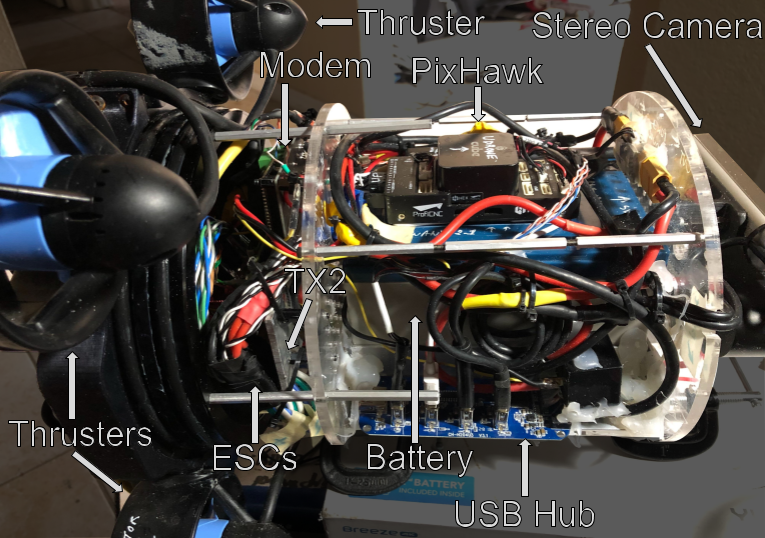
\includegraphics[width=\maxwidth{\textwidth}]{img/side_annotated.png}
\caption{Annotated Picture of uDrone without Enclosure}
\legend{\emph{Source}: Photo courtesy of Jnaneshwar Das, used with permission.}
\label{annotated}
\end{figure}

\section{Software}
In order to function as a testbed for innovation, the uDrone needed to be built using open source and easily accessible software. Additionally, it was desired to use the tools that the DREAMS lab had existing experience with.

\subsection{ROS}
All on board computers run Ubuntu Linux and the Robot Operating System (ROS). ROS is an open source library of tools that are commonly used for robotic systems. The architecture of ROS is similar to a network, consisting of nodes, processes that perform computation, and messages that communicate between notes \parencite{ros,ros-wiki}. All of the sensors, such as the ZED 2 and Ping Echosounder, have existing packages that can communicate with ROS. The sensor data is accessed via a node which generates messages that are used by other nodes. ROS has many additional libraries that are useful for autonomy and other uDrone needs.
% https://www.ros.org/
% http://wiki.ros.org/

\subsection{PX4}
The on board PixHawk flight controller runs PX4 on a nuttX operating system. PX4 is an open source autopilot for drones and other vehicles. This software is used and maintained by a series of academics and other drone developers. There is already a strong knowledge of PX4 from Dr. Das and other members of the DREAMS lab. At its most basic level, PX4 translates desired control inputs, i.e. go to a certain point or rotate clockwise, into specific motor actuation. It uses internal PID controllers to reach set points and mixer files to relate control inputs uniquely for different vehicles. Existing vehicle templates can be used to speed up development of a controller for the uDrone. Specifically, the HippoCampus micro AUV has a similar thruster configuration to the uDrone and was used as a starting point for development \parencite{px4}. 
% https://px4.io/

\subsection{MAVLink and MAVROS}
PX4 communicates using a protocol called MAVLink. There is a ROS package called MAVROS which allows for the translation between ROS messages and MAVLink messages. This package allows for users to write programs with ROS and communicate them directly to the flight controller without needing to write interpreters. This architecture was implemented for the uDrone to allow for fast and seamless development \parencite{mavros}.
% http://wiki.ros.org/mavros

\subsection{QGround Control}
In order to interact with the vehicle while it is running, a ground control software is used. For this project QGround Control is used. This software communicates with the flight controller running PX4 using MAVLink and can be used in both simulation and field trials. It can be used to test manual control, set various types of mission vehicles, and observe the state of the vehicle and all its components. In autonomous mode the vehicle is controlled directly from the on board ROS computer, but QGround Control allows for a window into its operation and provides control overrides when necessary \parencite{qgc}. 

\section{Simulation}
A core component of the whole system is the simulation environment. This allows for testing perception and control methodologies and forms the foundation of all the work that is eventually used on the uDrone. The goal of the simulation environment is to be as close to real life. A diagram showing how all the components of the simulation environment fit together can be seen in figure \ref{soft}. 

This particular setup is used because of its close resemblance to real world deployment. In simulation the control code, which runs with ROS on a desktop or OpenUAV container. In real world deployment this is all run on the internal CPU/GPU on-board the uDrone. The PX4 based flight controller is simulated using SITL while it is run on the PixHawk in deployment. And the simulated world in Gazebo is made to mimic the underwater world and vehicle dynamics that will be experienced in deployment. 

\begin{figure}
    \centering
    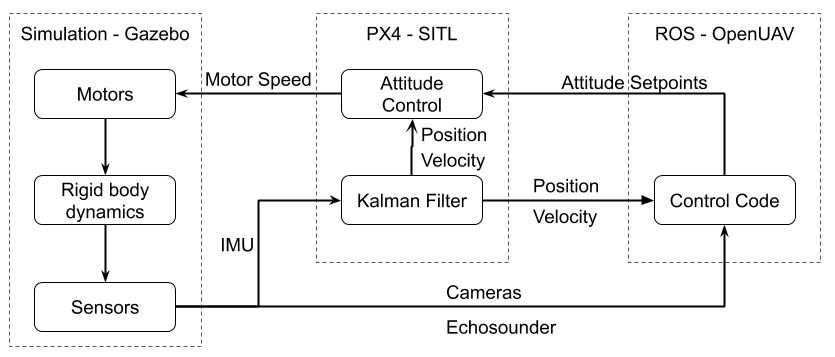
\includegraphics[width=\maxwidth{\textwidth}]{img/soft-sys.png}
    \caption{System diagram showing the interaction between the software components in simulation}
    \label{soft}
\end{figure}

\subsection{Gazebo}
A core component of the entire system is the simulation framework used for development and testing. The simulation of the uDrone is done using Gazebo. Gazebo is a simulator for robotics allowing for the testing of systems in real world like physical environments. It integrates directly with ROS, making development easier. Gazebo allows for the creation of custom worlds and robots, allowing for simulations of the uDrone on a coral reef. PX4 also has a library to work directly with Gazebo, which includes 3D and physics models for many of its vehicle templates. For most development, ROS is run and PX4 is emulated on the host system. Using this setup it is also possible to run hardware-in-the-loop simulations, allowing for tests of the performance of the TX2 and PixHawk Cube \parencite{gazebo}. 
% http://gazebosim.org/

\subsection{UUV Simulator}
To make the Gazebo environment as real as possible, a package called the Unmanned Underwater Vehicle Simulator (UUV Sim) was used to simulate the effects of a vehicle moving underwater. UUV Sim was specifically designed to aid in the simulation of underwater vehicles. This packages main contribution and reason it was used on this project is the implementation of the equations of motion detailed by Thor Forsson in the Handbook of Marine Hydrodynamics. It also has improved thruster models, several controllers purpose built for AUVs, aquatic world files, and several vehicle models \parencite{uuv}. 
% https://uuvsimulator.github.io/

% \subsection{Unity}
% While Gazebo is a very useful simulator for physics, other simulators are available for better photo-realism. As part of the uDrone project the Unity game engine was used in conjunction with Gazebo for better photorealism. In this setup, the two simulator environments act in a master-slave fashion. The vehicle position, orientation, and movement is controlled in Gazebo. This data is then sent to Unity, which moves the vehicle accordingly. The cameras are modeled in Unity and they send back data to ROS based on what they see in this simulation. Controllers in ROS then use this data to send control signals through PX4 back to Gazebo. For more information on this setup and its application, see Harish’s Thesis.

\subsection{Reef Data}

One of the main challenges to creating a simulation environment to test the uDrone was in finding a model of a reef to test with. To obtain a realistic reef model I took video footage while recreational scuba diving in Kona, Hawaii. This was a particularly good spot since the dives sites were only a few miles away from the planned initial site of the uDrone deployment. I built a special rig that allowed me to hold two GoPro cameras while I dove. The goal of the two cameras was to get a wider spread and possibly use them together as a stereo pair. Because the cameras were not synced, the stereo pair plan did not work.

The 3D model was generated from the footage using Agisoft Metashape structure from motion software. The videos, originally shot at 30 frames per second, needed to be down sampled to 6 frames per second. This allowed for some overlap between each image but not so much that processing took too long. Next, Agisoft found feature correspondence between the overlapping images. With this information, the software was able to generate a mesh and full 3D model with a photographic overlay, seen in figure \ref{reef}. 

\begin{figure}[h]
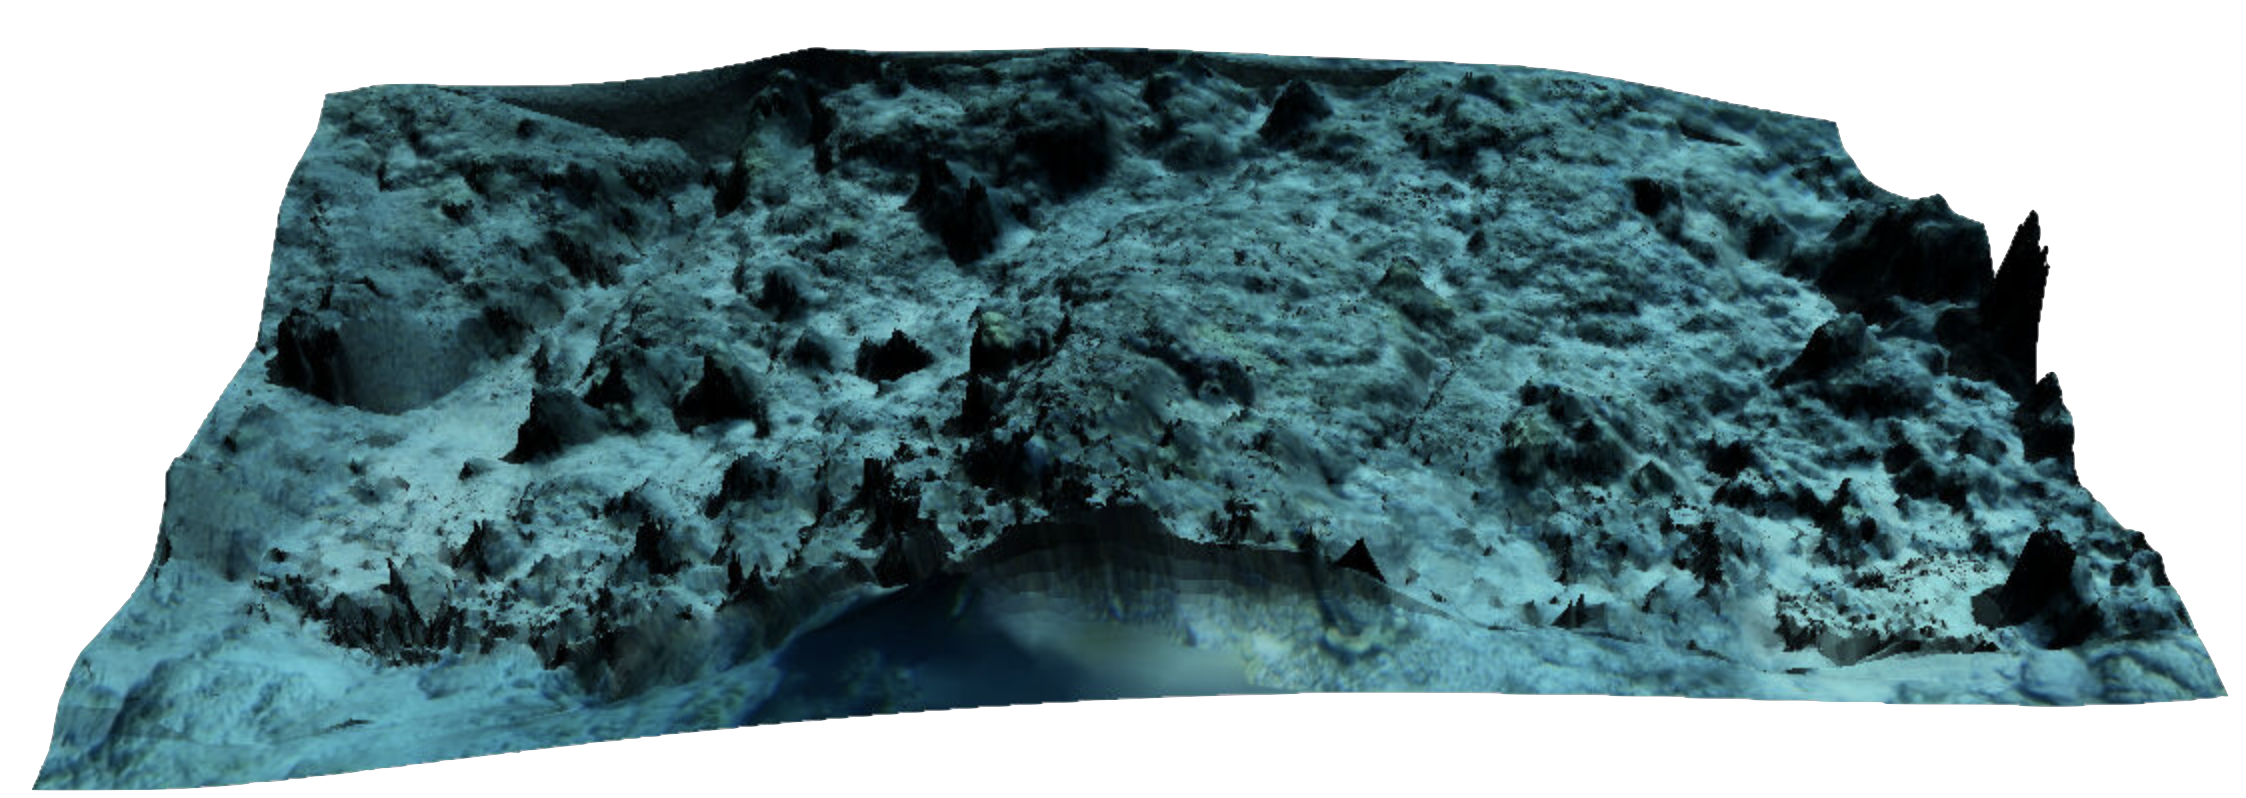
\includegraphics[width=\maxwidth{\textwidth}]{img/reef.png}
\caption{Three Dimensional Reef Model for Simulation}
\label{reef}
\end{figure}

This process was not without significant challenges. Since there are many suspended particles in the water, structure from motion would often mistake these for features and incorporate them into the surface. For this reason, although many videos were shot, only one was able to be turned into a reliable reef model. The 3D model came from a section of the Kaloko Arches dive site near Kona, Hawaii. While the exact dimensions cannot be determined using this method, the model is estimated to be 16 by 8 meters.

% This model served its purpose for early works and proof of concept. Later in the project we received much larger and higher fidelity reef models from Dr. John Burns at University of Hawaii in Hilo. As part of his reef monitoring and conservation studies, he and his team conduct thorough imaging surveys of sections of the reef and convert them into 3D models. These models are incorporated into the Unity simulation framework that is used for greater photorealism. 

% https://www.johnhrburns.com/


\section{Construction}
% The physical design and construction of the vehicle was led by an expert modeler and builder, Cole Brower. He was aided by an undergraduate, Rodney Staggers, Jr., working on a NASA Space Grant (***CHECK THIS***). First, rough drawings were generated by the stakeholders on the project. Using these sketches, the build team created a full 3D model of the vehicle, including all internal & external components. 

The internal frame that supported the batteries and other electrical equipment and the external coupling for the thrusters were 3D printed based on designs. The whole vehicle was then assembled and prepared for testing. By leveraging 3D printing the team was able to test our and rapidly prototype design ideas. Also, since the structural components are easier to source as they can be 3D printed almost anywhere. 

One major change that came about during this construction process involved the design of the interior structure. This structure went through several iterations in order to make physically working on the uDrone easier. Specifically, the compute cluster was repositioned so it would be closer to the camera in the front and easier to access without removing the batteries. Additionally, the entire structure was built to be removed as one solid piece, allowing for easy access when inserting into the enclosure. 


% \begin{itemize}
%     \item Constant Speed
%     \item Constant Distance to Reef
%     \item Carry Scientific Equipment
%     \item Easy to Deploy
% \end{itemize}

% \section{Design Motivation}
% \subsection{Background}
% Underwater vehicles and Underwater Propulsion methods
% \subsection{Quadcopters}
% Mimic design and control
% Leverage Drone infrastructure

% \section{Actuation}
% \subsection{Enclosure}
% \subsection{Thrusters}

% \section{Perception}
% \subsection{Acoustic Pinger}
% \subsection{ZED Stereo Camera}
% \subsection{Other Sensors}

% \section{Automation}
% \subsection{Background}
% \subsection{Pixhawk/Px4}
% \subsection{Tx2}
% \subsection{ROS}

